\documentclass{beamer}

\usepackage[utf8]{inputenc}
\usepackage[spanish]{babel}
\usepackage{graphicx}

\xdefinecolor{rojito}{rgb}{1,0.3,0.3}
\xdefinecolor{oliva}{cmyk}{0.64,0,0.95,0.4}
\xdefinecolor{minaranja}{rgb}{0.94,0.48,0.2}

\usetheme{Madrid}
\usecolortheme[named=rojito]{structure}

\title[Computación Cuántica]{Mutation testing para lenguajes cuánticos}
\author{Luis Aguirre \& Javier Pellejero}
\institute[UCM]{Universidad Complutense de Madrid\\ Facultad de Informática}

\newcommand{\filados}[2]{ \left. \begin{array}{c}	#1 \\	#2	 \end{array} \right. }
\newcommand{\filacuatro}[4]{ \left. \begin{array}{c}#1\\#2\\#3\\#4	\end{array} \right.}
\newcommand{\base}[1]{|#1\rangle}
\newcommand{\lbase}[1]{\langle#1|}
\newcommand{\dotproduct}[2]{\langle#1|#2\rangle}
\newcommand{\tensor}[2]{|#1\rangle\langle#2|}
\newcommand{\baseup}{\mid\uparrow\rangle}
\newcommand{\baseright}{\mid\rightarrow\rangle}
\newcommand{\baseupright}{\mid\nearrow\rangle}
\newcommand{\baseupleft}{\mid\nwarrow\rangle}
\newcommand{\transpose}[1]{#1 ^\dag}
\newcommand{\complex}{\mathbb{C}}
\newcommand{\puertai}{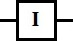
\includegraphics[scale=0.8]{imagenes/puertai}}
\newcommand{\puertax}{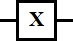
\includegraphics[scale=0.8]{imagenes/puertax}}
\newcommand{\puertay}{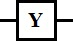
\includegraphics[scale=0.8]{imagenes/puertay}}
\newcommand{\puertaz}{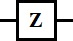
\includegraphics[scale=0.8]{imagenes/puertaz}}
\newcommand{\puertah}{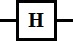
\includegraphics[scale=0.8]{imagenes/puertah}}
\newcommand{\puertacnot}{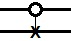
\includegraphics[scale=0.8]{imagenes/puertacnot}}
\newcommand{\eprpair}{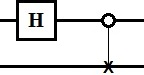
\includegraphics[scale=0.8]{imagenes/eprpair}}
\newcommand{\cnot}{C_{\mathrm{not}}}

\begin{document}

\begin{frame}
	\titlepage
	\begin{center} Doble Grado en Matemáticas e Ingeniería Informática\end{center}
\end{frame}

\begin{frame}
\frametitle{Índice}
	\tableofcontents
\end{frame}

\section{Introducción al testing}

\begin{frame}
	\frametitle{Breve introducción al testing}
	\begin{itemize}
	\item El testing es una disciplina orientada a aumentar la calidad y fiabilidad de un programa.
	\item Su principal objetivo es encontrar errores para de esta manera poder corregirlos.
	\item Sin embargo, el testing no nos permite demostrar que un programa no contiene errores! (\textit{E. W. Dijkstra. Notes On Structured
Programming (EWD249), Section 3, 1970})
	\end{itemize}
\end{frame}

\begin{frame}
	\frametitle{Breve introducción al testing}
	Es importante distinguir entre fault, error y failure:
	
	\begin{itemize}
	\item \textbf{Fault:} defecto estático en el código.
	\item \textbf{Error:} estado interno incorrecto durante la ejecución del programa.
	\item \textbf{Failure:} comportamiento externo incorrecto con respecto a los requisitos del programa.
	\end{itemize}
			
\end{frame}

\begin{frame}
	\frametitle{Breve introducción al testing}
	Un test se compone principalmente de 2 componentes:

	\begin{itemize}
	\item Los \textbf{valores de los inputs} que se necesitan para que se ejecute el programa.
	\item  El \textbf{resultado} que producirá el programa en caso de que se comporte correctamente.
	\end{itemize}
			
\end{frame}

\section{Mutation Testing}

\begin{frame}
	\frametitle{Mutation Testing}
	\begin{itemize}
	\item A diferencia del testing tradicional, el \textbf{mutation testing} nos permite conocer la efectividad de un conjunto de test.
	\item Por ello, el \textbf{mutation testing} parte de un programa que se comporta correctamente.
	\end{itemize}
\end{frame}

\begin{frame}
	\frametitle{Operador de mutación y mutante}
	\begin{itemize}
	\item Un \textbf{operador de mutación} es una regla que especifica una variación sintáctica sobre una cadena de la gramática del lenguaje del programa.
	\item Un \textbf{mutante} es el resultado de la aplicación de un \textbf{operador de mutación}.
	\end{itemize}
	Ejemplo: 
	\begin{table}[]
		\begin{tabular}{|l|l|}
		\hline
		Operador    & Operador de mutación  \\ \hline
		\textless{} & \textless{}=           \\ \hline
		\end{tabular}
	\end{table}
	
	\begin{table}[]
		\begin{tabular}{|l|l|}
		\hline
		Codigo Original     & Mutante                 \\ \hline
		if (x \textless{} 10) & if (x \textless{}= 10)  \\ \hline
		\end{tabular}
	\end{table}
	
\end{frame}
	
\end{document}
